\section{The theory of relators.}\label{sec:relators}
The lucid presentation in the notes \cite{benabou2000distributors} and in \cite[\S \textbf{4}]{Cordier2008}, \cite{Bor2} are standard references to follow this section. Our only merit here is having expressed several proofs using coend calculus. The arguments are essentially unchanged, and yet the employment of coends is implicit in \cite{benabou2000distributors}, and only partially spelled out in \cite{Bor2}.% Another classical reference is chapter 4 in \cite{Cordier2008}.
The lucid presentation in the notes \cite{benabou2000distributors} and in the book \cite[\S \textbf{4}]{Cordier2008} are standard references to follow this section. Our only merit here is that we have restated several proofs using coends; these arguments are somewhat implicit in \cite{benabou2000distributors} and only partially spelled out in \cite{Bor2}.
\def\Dist{\textbf{Relt}}
\begin{definition}[The bicategory of relators]\label{profdef}
There exists a bicategory $\Dist$ having
\begin{itemize}
\item 0-cells (objects) those of $\Cat$ (small categories $\A,\B,\C,\D,\dots$);
\item 1-cells $\proP,\proQ\dots$, depicted as arrows $\A\pto \B$, the functors $\A^\opp\times\B\to \Sets$;
\item 2-cells $\alpha\colon\proP\Rightarrow\proQ$ the natural transformations between these functors.
\end{itemize}
Given two contiguous 1-cells $\A\stackrel{\proP}{\pto}\B\stackrel{\proQ}{\pto}\C$ we define their \emph{composition} $\proQ \diamond \proP$ as the coend
\[
\proQ \diamond \proP(a,c) := \int^{x\in\B} \proP(a,x)\times\proQ(x,c)
\]
\end{definition}
\begin{definition}
This definition works well also with $\Sets$ replaced by an arbitrary Bénabou cosmos $\V$, \ie in any symmetric monoidal closed and bicomplete category: in this case we speak of $\V$-relators in the bicategory $\Dist(\V)$.
\end{definition}
\begin{remark}[Naming a category]
The 1-cells of $\Dist$ are more often called \emph{profunctors} or \emph{distributors} (\cite{benabou2000distributors} follows the equation $\text{funct\emph{ions}} : \text{funct\emph{ors}} = \text{distribut\emph{ions}} : \text{distribut\emph{ors}}$), \emph{correspondences} (consider the case when $\V=\{0,1\}$ \ie where $\A, \B$ are sets regarded as discrete categories), or \emph{bimodules} (consider the case where $\V=\cate{Ab}$ and $\A,\B$ are rings; see \cite{nashphd} and several examples below).

As we will see during the present section, the bicategory $\Dist$ carries a fairly rich structure: it is then quite difficult to choose a name for its 1-cells able to convey this richness or the main features thereof. 

There are several reasons why most of the above choices are unsatisfying: naming the 1-cells of $\Dist$ ``profunctors'' may generate confusion as the prefix \emph{pro-$\C$} denotes the pro-completion of a category $\C$, \ie the collection of all ``formal'' cofiltered limits of objects of $\C$; then a pro-functor, etymologically, should be an object of the pro-completion of some functor category, which is not true; justifying the name ``distributor'' would request a more strict analogy between $\proP \colon \A \to \B$ and distributions in mathematical analysis; \emph{correspondence} is a name so inflated that it doesn't conveys any intuition at all;\dots

While taking note of this situation, we decide to add a new term to this vast zoology, and we call the 1-cells of $\Dist$ ``relators'', motivated by the analogy in the following example.
\end{remark}
\begin{example}[Relators as generalized relations]
A relator between $\{0,1\}$-categories is a function between sets $A^\opp\times B\to \{0,1\}$, namely a function $A\times B \to \{0,1\}$, or in other words a relation regarded as a subset $R\subseteq A\times B$.

From this point of view, relators $\A\pto \B$ can be thought as \emph{generalized relations}, taking values in more complicated, or structured, enriching cosmoi. This point of view is what Lawvere \cite[\S\textbf{4},\textbf{5}]{LawvereFW:metsgl} calls \emph{generalized logic}, and it regards the coend in \adef \refbf{profdef}, and the product $\proP(a,x)\times \proQ(x,b)$ therein, as a generalized existential quantification and a generalized conjunction respectively, giving a composition rule for generalized relations: the coend stands as
\[
(x,z)\in R\circ S \iff \exists y\in Y : \big((x,y)\in R\big)\land \big((y,z)\in S\big)
\]
for two relations $R\subseteq X\times Y, S\subseteq Y\times Z$: we can depict this analogy as in Figure \refbf{fig:profuncs}: this is valid for suitable relations $R\colon X\pto Y$ and $S\colon Y\pto Z$ or suitable relators $\textsc{r}\colon \cate{X}\pto \cate{Y}$ and $\textsc{s}\colon \cate{Y}\to\cate{Z}$.
\end{example}
\begin{center}
\begin{figure}[h!]
\label{fig:profuncs}
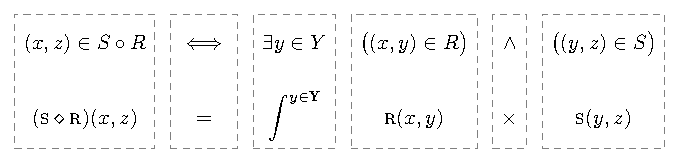
\includegraphics[scale=1]{figures/fig21}
\caption{The analogy between the composition of relators between categories and the composition of relations between sets gives rise to what lawvere calls \emph{generalized logic}.}
\end{figure}
\end{center}
\begin{example}
Let $A,B$ be sets, considered as categories having only identity arrows via the embedding $\Sets\subset\Cat$. A relator $A\pto B$ is then simply a collection of sets $P_{ab}$, one for each $a\in A,b\in B$. Their composition then results in a ``categorified'' matrix multiplication, in that the coend simplifies to be a mere coproduct: given $\proP\colon A\to B$, $\proQ\colon B\to C$ we have
\[
(\proP\diamond \proQ)_{ac} = \coprod_{b\in B}P_{ab}\times Q_{bc}
\]
if $P_{ab}=\proP(a,b)$ and $Q_{bc}= \proQ(b,c)$.
\end{example}
\begin{remark}\label{alternative}
There is an alternative, but equivalent definition for $\proQ \diamond \proP$ which exploits the universal property of $\widehat{\C}$ as a free cocompletion: any relator $\proP\colon \A\pto \B$ can be identified with its \emph{mate} under the adjunction giving the cartesian closed structure of $\Cat$,
\[
\Fun(\A^\opp\times \B ,\Sets)\cong \Fun(\B, [\A^\opp,\Sets])
\]
\ie with a functor $\widehat\proP\colon\B\to \widehat{\A}$ obtained as $b\mapsto \proP(\firstblank,b)$. Hence we can define the composition $\A\stackrel{\proP}{\pto}\B\stackrel{\proQ}{\pto}\C$ to be $\Lan_\yon \widehat\proP\circ\widehat\proQ$:
\[\xymatrix{
& \B \ar[d]_{\yon }\ar[r]^{\widehat\proP}& \widehat{\A} \\
\C \ar[r]_{\widehat\proQ}& \widehat{\B} \ar[ur]_{\Lan_\yon \widehat\proP}& 
}\]
\end{remark}
This is equivalent to the previous definition, in view of the characterization of a left Kan extension as a coend in $\widehat{\A}$, given in Equation \refbf{kanend}:
\[\Lan_\yon \widehat\proP\cong \int^b\widehat{\B}(\yon_b,\firstblank)\cdot \widehat\proP(b).\] 
Since in $\Sets$ copower coincides with product (\ie $X\cdot Y\cong X\times Y$, since $\Sets(X\cdot Y,B)\cong \Sets(X,\Sets(Y,B))\cong \Sets(X\times Y,B)$, naturally in $B$), we have
\begin{align*}
\Lan_\yon \widehat{\proP}(\widehat{\proQ}(c)) &\cong \int^b \widehat{\B}(\yon_b,\widehat{\proQ}(c))\cdot \widehat{\proP}(b)\\
&\cong \int^b \widehat{\proQ}(c)(b)\cdot \widehat{\proP}(b)\\
&\cong \int^b \proP(\firstblank,b)\times \proQ(b,c).
\end{align*}
\begin{remark}\label{profundefs}
The properties of (strong) associativity and unitality for the composition of relators follow directly from the associativity of cartesian product, its cocontinuity as a functor of a fixed variable, and from the ninja Yoneda lemma \refbf{ninjayo}, as shown by the following computation:
\begin{itemize}
\item Composition of relators is associative (up to isomorphism), giving the \emph{associator} of a bicategory structure:
\begin{align*}
\proP \diamond (\proQ \diamond \proH) &=\int^x\proP(b,x)\times (\proQ \diamond \proH)(x,a)\\
&=\int^x \proP(b,x)\times\Big( \int^y \proQ(x,y)\times\proH(y,a)\Big)\\
&\cong \int^{xy}\proP(b,x)\times\Big( \proQ(x,y)\times\proH(y,a)\Big)\\
(\proP \diamond \proQ) \diamond \proH &= \int^x(\proP \diamond  \proQ)(b,x)\times\proH(x,a)\\
&\cong \int^{xy}\Big(\proP(b,y)\times\proQ(y,x)\Big)\times\proH(x,a)
\end{align*}
and these results are clearly isomorphic, and naturally so, once we changed name to ``integration'' variables (which are obviously ``mute''). See Remark \refbf{isitpentagon} below for a discussion on the coherence laws of this associator.
\item Any object $\A$ has an identity arrow, given by the ``diagonal'' relator $\A(\firstblank,\secondblank)=\hom_{\A}\colon \A^\opp\times \A\to \Sets$: the fact that $\proP \diamond \hom\cong\proP$, $\hom \diamond\, \proQ\cong\proQ$ simply rewrites the ninja Yoneda lemma.
\end{itemize}
\end{remark}
\begin{remark}\label{isitpentagon}
The isomorphism above is part of the data turning $\Dist$ into a bicategory; the \emph{associator} realizes the identification between different parenthesizations of 1-cells, and the \emph{unitor} realizes the identification between $\proP\diamond \hom\cong \proP$.

To ensure that ``every'' diagram which can be constructed from these data commutes some coherence conditions have to be imposed. One of these is the \emph{pentagon} identity \cite{McL}, encoded in the following diagram:
\begin{center}
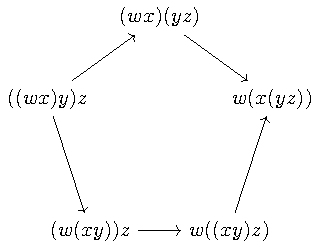
\includegraphics[scale=1]{figures/fig22}
\end{center}
This equality is natural in each argument (as a consequence of being a composition of natural transformations). 

It's immediate to observe that the validity of the pentagon identity in the case of the cartesian monoidal structure of $\Sets$, and the naturality thereof, ensure that the associator (whose components are) $(\proP\diamond\proQ)\diamond\proH \Rightarrow \proP\diamond(\proQ\diamond\proH)$ satisfies the pentagon identity; a similar argument shows that the unitor satisfies similar (left and right) triangular identities, as a consequence of the naturality of the ninja Yoneda lemma \refbf{ninjayo}.
\end{remark}
\begin{definition}[Einstein notation]\label{einstein}
There is a useful notation which can be implied to shorten involved computations with coends, and which is particularly evocative when dealing with relators; we choose to call it \emph{Einstein convention} for evident graphical reasons.\footnote{This notation has been adopted also in the beautiful \cite{emilyreedy}, a valuable reading for several reasons, last but not least the fact that its authors adopt some coend-fu to simplify the discussion about ``Reedy calculus''.}

Let $\proP\colon \A\pto \B$, $\proQ\colon \B\pto\C$ be two composable relators. If we adopt the notation $\proP^a_b, \proQ^b_c$ to denote the images $\proP(a,b), \proQ(b,c)\in\Sets$ (keeping track that superscripts are contravariant and subscripts are covariant components), then composition of relators acquires again the form of a ``matrix product'':
\[\textstyle 
\proP\diamond \proQ(a,c) = \int^b \proP^a_b\times \proQ^b_c = \int^b \proP^a_b \proQ^b_c.
\]
From now on, we feel free to adopt the Einstein summation convention during long calculations.
\end{definition}

\begin{remark}[(Co)presheaves are relators]
Presheaves on $\C$ obviously correspond to relators $\C\pto\cate{1}$; copresheaves, \ie functors $\C\to \Sets$, correspond to relators $\cate 1\pto\C$.
\end{remark}
\subsection{Embeddings and adjoints}
There are two identity-on-objects embeddings $\Cat\to\Dist$ (respectively the \emph{covariant} and the \emph{contravariant} one, looking at the behaviour on 2-cells), and send a diagram in $\Cat$ respectively to
\[
\xymatrix@R=5mm@C=3mm{
\C \ar@/_1pc/@<-3pt>[dd]_F\ar@/^1pc/@<3pt>[dd]^G & {\scriptsize\boxed{\Cat^\opp\to \Dist}}& \C\ar@/_1pc/@<-3pt>@{<-}[dd]_{\proP_F}\ar@/^1pc/@<3pt>@{<-}[dd]^{\proP_G} \\
&\mapsto& \\
\D && \D 
\ar@{=>}(-3,-10);(3,-10)^\alpha
\ar@{=>}(30,-10);(36,-10)^{\proP_\alpha}
}
\qquad\quad\quad
\xymatrix@R=5mm@C=3mm{
\C \ar@/_1pc/@<-3pt>[dd]_F\ar@/^1pc/@<3pt>[dd]^G & {\scriptsize\boxed{\Cat^\text{co}\to \Dist}}& \C \ar@/_1pc/@<-3pt>[dd]_{\proP^F}\ar@/^1pc/@<3pt>[dd]^{\proP^G} \\
&\mapsto& \\
\D && \D 
\ar@{=>}(-3,-10);(3,-10)^\alpha
\ar@{<=}(30,-10);(36,-10)^{\proP^\alpha}
}
\]
This clearly defines a (pseudo)functor, since it's easy to see that
\begin{itemize}
\item $\proP_{FG}\cong \proP_F \diamond \proP_G$, and $\proP^{FG}\cong \proP^G \diamond \proP^F$;
\item $\proP_{\id_{\A}}=\proP^{\id_{\A}}=\A(\firstblank,\secondblank)$.
\end{itemize}
Natural transformations $\alpha\colon F\Rightarrow G$ are obviously sent to 2-cells in $\Dist$, and the covariancy of this assignment is uniquely determined as in the diagram above.
\begin{remark}\label{theyre.adjoints}
The 1-cells $\proP_F$, $\proP^F$ are not independent: they are \emph{adjoint} 1-cells in the bicategory $\Dist$. Indeed, for every $F\in \Cat(\A,\B)$ we can define 2-cells
\begin{gather}
\xymatrix{
\epsilon = \epsilon_F\colon \proP_F \diamond \proP^F \ar@{=>}[r] & \B(\firstblank,\secondblank)
}\\
\xymatrix{
\eta = \eta_F\colon \A(\firstblank,\secondblank)\ar@{=>}[r] & \proP^F \diamond \proP_F
}
\end{gather}
(\emph{counit} and \emph{unit} of the adjunction): here we unravel the coends involved in these definitions.
\begin{itemize}
\item For what concerns the counit, we  write the coend $\proP_F \diamond \proP^F$ as the quotient set
\[
\int^x \B(a, Fx)\times \B(Fx,b) = \Big(\coprod_{x\in \A} \B(a, Fx)\times \B(Fx,b)\Big)/\!\simeq
\]
where $\simeq$ is the equivalence relation generated by $\big(a\xto{u}Fx,Fx\xto{v}b\big)\simeq\big(a\xto{u'}Fy,Fy\xto{v'}b\big)$ if there is $t\colon x\to y$ such that $v'=Ft\circ v$ e $Ft\circ u=u'$. This can be visualized as the commutativity of the square
\[
\xymatrix@R=3mm@C=8mm{
& Fx \ar@{.>}[dd]^{Ft}\ar[dr]^v& \\
a \ar[dr]_{u'}\ar[ur]^u&& b \\
& Fy\ar[ur]_{v'} &
}
\] Now it's easily seen that sending $\big(a\xto{u}Fx,Fx\xto{v}b\big)$ in the composition $v\circ u$ descend to the quotient with respect to $\simeq$, hence $\epsilon\colon \proP_F \diamond \proP^F \to \B(\firstblank,\secondblank)$ is well defined. All boils down to notice that the composition
\[
c\colon \B(a, Fx)\times \B(Fx,b)\to \B(a,b)
\]
defines a cowedge in the variable $x$.
\item The unit of the adjunction is the 2-cell
\[
\xymatrix{
\eta\colon \A(\firstblank,\secondblank)\ar@{=>}[r] & \proP^F \diamond \proP_F
}
\]
obtained when we noticed that $\proP^F\ccirc\proP_F(a,b) = \int^X \B(Fa,x)\times\B(x,Fb)\cong \B(Fa,Fb)$ (as a consequence of the ninja Yoneda lemma), is simply determined by the action of $F$ on arrows, $\A(a,b)\to \B(Fa,Fb)$.
\end{itemize}
We now have to verify that the zig-zag identities (see \cite[Thm\@.\textbf{3.1.5.(2)}]{Bor1}) hold: 
\begin{gather*}
(\proP^F\ccirc\epsilon)\circ (\eta\ccirc \proP^F) = \id_{\proP^F}\\
(\epsilon\ccirc \proP_F)\circ(\proP_F\ccirc \eta) = \id_{\proP_F}
\end{gather*}
As for the first, we must verify that the diagram
\[
\xymatrix@C=1.5cm{
\proP^F \ar[r]^\sim\ar@{=}[d] & \B(\firstblank,\secondblank)\ccirc\proP^F \ar[r]^{\eta\ccirc\proP^F}& (\proP^F\ccirc\proP_F)\ccirc\proP^F \ar[d]^\cong\\
\proP^F & \ar[l]^\sim \proP^F\ccirc\B(\firstblank,\secondblank) & \ar[l]^{\proP^F\ccirc\epsilon} \proP^F\ccirc(\proP_F\ccirc\proP^F)
}
\]
commutes. One has to send $h\in \proP^F(u,v)=\B(Fu,v)$ in the class $[(\id_u,h)]\in \int^x\B(u,x)\times \B(Fx,v)$, which must go under $\eta\ccirc \proP^F$ in the class $[(F(\id_u),h)]\in \int^{xy}\B(Fa,x)\times\B(x,Fy)\times \B(Fy,b)$, canonically identified with $\int^y\B(Fa,Fy)\times \B(Fy,b)$. Now $\proP^F\ccirc\epsilon$ acts composing the two arrows, and one obtains $F(\id_A)\circ h=h$ back.

Similarly, to prove the second identity, the diagram
\[
\xymatrix@C=1.5cm{
\proP_F \ar[r]^\sim\ar@{=}[d]& \proP_F\ccirc\B(\firstblank,\secondblank) \ar[r]^{\proP_F\ccirc\eta}& \proP_F\ccirc(\proP^F\ccirc\proP_F) \ar[d]^\cong\\
\proP_F & \ar[l]^\sim\B(\firstblank,\secondblank)\ccirc\proP_F & \ar[l]^{\epsilon\ccirc\proP_F}(\proP_F\ccirc\proP^F)\ccirc\proP_F
}
\]
must commute (all the unlabeled isomorphisms are the canonical ones). This translates into
\[
\xymatrix{
\Big(a\xto{u}Fb\Big) \ar@{|->}[r]& (u, \id_b)_\sim \ar@{|->}[r]& (u, F(\id_b)) \ar@{|->}[r]& u\circ F(\id_b)=u,
}
\]
which is what we want; hence $\proP_F\dashv \proP^F$. \qed
\end{remark}
\begin{remark}
Two functors $F\colon \A\leftrightarrows \B\colon G$ are adjoints if and only if $\proP_F\cong \proP^G$ (and therewith $G\dashv F$) or $\proP_G\cong \proP^F$ (and therewith $F\dashv G$).
\end{remark}
\begin{remark}
It is a well-known fact (see \cite[dual of Prop. \textbf{3.4.1}]{Bor1}) that if $F\dashv G$, then $F$ is fully faithful if and only if the unit of the adjunction $\eta\colon 1\to GF$ is an isomorphism.

This criterion can be extended also to functors which do not admit a ``real'' right adjoint, once noticed that $F$ is fully faithful if and only if $\A(a,b)\cong \B(Fa,Fb)$ for any two $a,b\in \A$, \ie if and only if the unit $\eta\colon \hom_{\A}\Rightarrow \proP^F\ccirc\proP_F$ is an isomorphism.
\end{remark}
\begin{example}
Given a relator $\proP\colon \A\pto \B$ and a functor $F\colon \B\to \D$ we can define $\proP\otimes F$ to be the functor $\A\to \D$ given by $\Lan_{y}F\circ\widehat{\proP}$ (provided this colimit exists), where $\widehat\proP\colon \B\to\widehat{\A}$ is the adjunct of $\proP$. 

More explicitly, 
\[
\proP\otimes F(a) = \int^b \Nat(\yon_b,\proP(\firstblank,a))\cdot Fb\cong \int^b \proP^b_a\cdot F_b
\]
Exploiting this definition, several things can be proved via coend-fu:
\begin{itemize}
\item $\hom_{\B}\otimes F\cong F$ as a consequence of the ninja Yoneda lemma;
\item If $\C\stackrel{\proQ}{\pto}\A\stackrel{\proP}{\pto} \B\xrightarrow{F}\cate{X}$, then $(\proP\diamond \proQ)\otimes F\cong \proQ\otimes(\proP\otimes F)$: indeed
\begin{align*}
[(\proP\diamond \proQ)\otimes F]a & = \int^b (\proP\ccirc\proQ)^b_a\times F_b \\
&\cong \int^{bx}\proP^b_x\times \proQ^x_a\times F_b\\
&\cong \int^x\proQ^x_a \times\Big( \int^b\proP^b_x \times F_b \Big)\\
&\cong \int^x\proQ^x_a \times (F\otimes\proP)_x = [\proQ\otimes(\proP\otimes F)]a
\end{align*}
\end{itemize}
\end{example}
\begin{example}[Kan extensions in $\Dist$]
Any relator $\proP$ has a right Kan extension $\Ran_\proP$ in the sense that the notion has in any bicategory, where composition of functors or natural transformations is replaced by composition of 1- or 2-cells.

One has the following chain of isomorphisms in $\Dist$ (see Definition \refbf{einstein} for the Einstein convention):
\begin{align*}
\Nat(\proG\ccirc\proP,\proH) &\cong \int_{ab}\Sets\big( (\proG\ccirc \proP)^a_b,\proH^a_b \big)\\
&\cong \int_{ab} \Sets\Big( \int^x \proG^a_x \times \proP^x_b ,\proH^a_b\Big)\\
&\cong \int_{abx}\Sets\big( \proG^a_x,\Sets(\proP^x_b,\proH^a_b) \big)\\
&\cong \int_{ax}\Sets\Big( \proG^a_x,\int_b\Sets(\proP^x_b,\proH^a_b)\Big)\\
&\cong \int_{ax}\Sets\Big( \proG^a_x,\Ran_\proP\proH^a_x\Big)\\
&\cong \Nat(\proG,\Ran_\proP\proH)
\end{align*}
when we define $\Ran_\proP\proH(a,x)$ to be $\Nat\big(\proP(x,\firstblank),\proH(a,\firstblank)\big)$.
\end{example}
% \subsection{The Yoneda structure on $\Cat$ and $\Dist$}
% Before we begin, we must familiarize with \emph{Kan liftings}: in the same way a (global) Kan extension consists in an adjoint to the inverse image functor $p^*$ (see Def \refbf{kann}), a (global) Kan \emph{lifting} consists of an adjoint to the \emph{direct} image functor $p_*$. The definition is best appreciated in a general bicategory.
% \begin{definition}[Kan liftings]
% Let $\mathcal{K}$ be a bicategory. Given 1-cells $p\colon B \to C$, $f\colon A \to C$ in $\mathcal{K}$, a \emph{right Kan lift} of $f$ through $p$, denoted $\Rift_p f$, is a 1-cell $\Rift_p(f)\colon A \to B$ equipped with a 2-cell 
% \[
% \varepsilon: p \circ \Rift_p(f) \Rightarrow f
% \]
% satisfying the following universal property: given any pair $(g\colon A \to B, \proH\colon p \circ g \Rightarrow f)$, there exists a unique 2-cell 
% \[
% \zeta: g \Rightarrow \Rift_p(f)
% \]
% such that the following diagram of 2-cells commutes for a unique $\zeta\colon g\Rightarrow \Rift_p(f)$
% \[
% \xymatrix{
%  & B \ar[dr] & \\
% A \ar@/^1.5pc/[ur]^g \ar[rr] && C
% \ar@{=>}(13,-4);(13,-11)^\proH
% } \qquad \text{\large =}\qquad  
% \xymatrix{
%  & B \ar[dr] & \\
% A \ar@/^2pc/[ur]^g \ar[ur]|{\Rift_p(f)} \ar[rr] && C
% \ar@{=>}(13,-4);(13,-11)^\epsilon
% \ar@{:>}(3,-1);(7,-5)^\zeta
% }
% \]
% \ie there is a unique factorization $\varepsilon \circ (p \ast \zeta) = \proH$. Dually, there exists a notion of \emph{left} Kan lift of $f$ through $p$, with all 2-cells going in the opposite direction, called $\Lift_pf$. 
% \end{definition}
% Now consider the diagram $\widehat{\A} \xot{\yon_{\A}} \A\xto{F} \B$, where $F\colon \A\to \B$ is a functor to a cocomplete category, so that the nerve-realization paradigm (see  Proposition \refbf{nervereal}) applies, and $\yon_{\A}\colon \A\to \widehat{\A}$ the Yoneda embedding. Then we can show that:
% \begin{enumerate}[label=\textbf{\roman*})]
% \item $\Lan_{\yon_{\A}}F\dashv \Lan_F \yon_{\A}$ (another form of the \textsc{nr}-paradigm);
% \item $F(-)\cong \Lift_{\B(F\firstblank,\secondblank)}y$ where ``Lift'' is the left Kan lifting of $y$ with respect to $\B(F\firstblank,\secondblank)$;
% \item $\Lan_{\yon_{\A}}\yon_{\A}\cong \id_{\widehat{\A}}$ (\ie, the Yoneda embedding is \emph{dense});
% \item In the diagram 
% \[\xymatrix@C=1.3cm@R=1.3cm{
% & \widehat{\A} \ar@{<-}[r]^{\Lan_{\yon F}\yon } & \widehat{\B} \\
% \A \ar[r]_F \ar[ur]^{\yon_\A}  & \B \ar[ur]_{\yon_\B} \ar[rr]_G && \C\ar[ul]_{\Lan_G\yon }
% \ar@{=>} (12,-15);(22,-5)
% \ar@{=>} (32,-10);(42,-10)
% }\]
% filled by canonical 2-cells, the arrow $\Lan_{\yon_{\A} \circ F}\yon_{\A}\circ \Lan_G\yon_{\A}$ coincides with $\Lan_{GF}\yon_{\A} (\cong \Lan_G\Lan_F \yon_{\A})$.
% \end{enumerate}
% \begin{proof}
% Let's begin by showing property (i). We have to prove that $\Lan_F\yon_{\A}\cong (B\mapsto {\B}(F\firstblank,B))$ (by uniqueness of adjoints). This is immediate if we write
% \begin{align*}
% \Lan_F\yon_{\A} (b) & \displaystyle \cong \int^a {\B}(Fa,b)\cdot \yon_{\A}(a)\\
% &\cong \displaystyle \int^a {\B}(Fa,b)\times {\A}(\firstblank,a)\\
% &\cong {\B}(F\firstblank,b)
% \end{align*}
% where the first isomorphism recognizes the $\Sets$-tensoring of $\Sets$ as the cartesian product, and the second is motivated by the ninja Yoneda lemma.

% To show property (ii), we have to prove that using $N_F$ as a shorthand for the functor $\Lan_F\yon_{\A}={\B}(F\firstblank,\secondblank)$, weh ave that $\Lift_{N_F}\dashv N_{F,*}$, where $N_{F,*}\colon P\mapsto N_F\circ P$for any $P\colon \A\to B$. We have that
% \begin{align*} 
% [{\A},\widehat{\A}]\big( \yon_{\A}, N_F\circ P \big) &\cong \int_{a'}\widehat{\A}\big(  \yon_{\A,a'}, N_F\circ P(a')\big)\\ 
% &  \cong \int_{a'}\widehat{\A}\big(  \yon_{\A,a'}, {\B}(F\firstblank,Pa')\big)\\
% &\cong \int_{a'}{\B}(Fa',Pa')\\
% &\cong [{\A,\B}](F,P)
% \end{align*}
% by the very definition of $N_F$ and by Proposition \refbf{naturalu}.

% Property (iii) again follows from the coend-form for the left Kan extension, and from the ninja Yoneda lemma.

% At this point property (iv) can be left as an exercise for the reader: it's enough to check that the functor $c\mapsto \Big( a\mapsto \Nat\big( \yon_{\B, Fa}, \Lan_G \yon_{\B}(c) \big) \Big)$ corresponds, by Yoneda lemma, to $ \Lan_G \yon_{\B}(c)(Fa)$, namely to ${\B}(GFa,c)$, namely to $N_{GF}(c)(a)$.\footnote{The reader puzzled by the multiplication of variables on which these functors depend could be relieved by a moderate use of $\lambda$-notation; we refrain to do so since the author spent a lot of time thinking how to render the $\firstblank$ and $\secondblank$ commands.}
% \end{proof}
% The above arguments sketches the proof that $\Cat$ is endowed with a canonical choice of a \emph{Yoneda structure} in the sense of \cite{street1978yoneda}.
% % \subsection{The compact closed bicategory $\Dist$.}
% % \trans{TODO!!1!}
% % \cite{cattani2005relators} investigates the structure of \emph{monoidal bicategory} (in the sense of \cite{stay2013compact}) of the bicategory $\Dist$; this decategorifies to the statement that the category $\textsf{Alg}(R)$ of \emph{algebras} over a ring $R$ is a monoidal bicategory, where
% \begin{itemize}
% \item 0-cells are $R$-algebras, \ie monoids in the category of $R$-modules;
% \item 1-cells $T\to S$ are bimodules ${}_T M_S$;
% \item 2-cells are bimodules maps $\alpha\colon {}_T M_S\to {}_T N_S$.
% \end{itemize} 
% We address the readers to \cite{stay2013compact} to see all the axioms and coherence conditions for a compact closed bicategory (see \adef \textbf{9-11} in particular) The monoidal bicategory structure on $\Dist$ is defined starting from the following data:
% \begin{itemize}
% \item 
% \item 
% \item 
% \item 
% \end{itemize}
% We now concentrate on an interesting interaction between co/end calculus and this compact closed structure on $\Dist$, following a MO comment \ci
% ùte{trimble-coends}.
\begin{remark}[The multibicategory of relators]
The bicategory of relators can be promoted to a \emph{multibicategory} in the sense of \cite[\textbf{1.4}]{cockett2003morphisms}; this means that we exploit the (partial) monoidal structure on each $\Dist(\C,\D)$ to specify a class of multimorphisms $\eta \colon \proP_1,\dots, \proP_n \pto \proQ$, depicted as diagrams
\[
\xymatrix{
X_0 \ar@/_4pc/[rrr]|-@{|}_{\proQ}
\ar[r]|-@{|}^{\proP_1} & X_1 \ar[r]|-@{|}^{\proP_2} & \dots \ar[r]|-@{|}^{\proP_n} & X_n
\ar@{=>}(22.5,-3);(22.5,-12)_{\eta}
}
\]
and composition, associativity and unitality thereof, follow at once from pasting laws for 2-cells in 2-categories \cite{kelly1982basic} (try to outline them as a straightforward exercise).
\end{remark}
% \subsection{Additional structure on $\Dist$.}
% Monoidal, symmetric monoidal and $S$-distributors from \cite{gambo-joy}. Model relators.
\begin{exerciseset}
\begin{exercisepoints}
\item Describe relators between monoids, regarded as one-object categories; describe relators between posets regarded as thin categories.
\item Given relators $\proK\colon \C\pto \D$ and $\proL\colon \C\pto\cate{E}$ define
\begin{gather*}
\proK\rhd \proL = \int_c [\proK(c,\firstblank), \proL(c,\secondblank)] 
\end{gather*}
Show that this operation is a Kan lifting (of $\proL$ along $\proK$); dually, given $\proH \colon \D\pto \A$ and  $\proL\colon \cate E\pto \A$ we can define 
\[
\proL\lhd \proH = \int_a [\proH(=,a), \proL(\firstblank,a)].
\]
Show that this second operation is a Kan extension (some vagueness is intended to be fixed as part of the exercise), and that these two operations ``behave like an action'' on $(\Dist,\ccirc,\hom)$ on the bicategory $\Dist$:
\begin{enumerate}[label=\textbf{\roman*})]
\item $(\proK\ccirc \proH)\rhd \proL\cong \proK\rhd(\proH\rhd \proL)$;
\item $\proL \lhd(\proK \ccirc \proH)\cong (\proL\lhd \proK)\lhd \proH$;
\item $\hom\rhd \proL\cong \proL\cong \proL\lhd \hom$.
\end{enumerate}
This is a na\"ive way to see that the structure on $\Dist$ given by $\diamond$ is \emph{biclosed} (\ie, $\diamond$ is a bifunctor $\Dist(\A,\B)\times \Dist(\B,\C) \to \Dist(\A,\C)$ and each $\proP\diamond\firstblank$, as well as each $\firstblank\diamond \proQ$ have right adjoints).
\item The \emph{collage} of two categories $\A,\B$ along a relator $\proP\colon \A \pto \B$ is defined to be the category $\A \uplus_\proP \B$ with the same objects as $\A \amalg \B$ and morphisms given by the rule
\[
\A\uplus_\proP \B(x,y) =
\begin{cases}
\A(x,y) & \text{ if } x,y\in\A\\
\B(x,y) & \text{ if } x,y\in \B\\
\proP(x,y) & \text{ if } x\in \A, y\in\B
\end{cases}
\]
and empty in every other case. Show that $\A\uplus_\proP \B$ has the universal property of the category of elements of $\proP$, regarded as a presheaf.
\item Show that the composition laws $\proP(A,B)\times \B(B,B')\to \proP(A,B')$, $\A(A,A')\times \proP(A',B)\to \proP(A, B)$ of arrows in $\A\uplus_\proP \B$ are governed by the universal property of a coend.
\item The \emph{cocomma object} $(F/G)$ of two functors $\cate{X} \xot{F} \A \xto{G} \cate{Y}$ is defined to be the pushout of
\[
\xymatrix{
	\A \amalg \A \ar[d]\ar[r]& \A \times \Delta[1] \\
	\cate{X} \amalg \cate{Y} & 
}
\]
in $\Cat$, where the horizontal arrow is the ``cylinder'' embedding. Show that $(F/G)$ is the collage of $\cate{X}$ and $\cate{Y}$ along the relator $\proP^G \ccirc \proP_F \colon \cate{X} \pto \cate{Y}$.
\item Given relators $\A \overset{\proP}\pto \B \overset{\proQ}\pto \C$ consider the categories $\A\uplus_\phi\B$ and $\B\uplus_\psi\C$. Describe the pushout
\[
\xymatrix{
\B \ar[r]\ar[d]& \A\uplus_\phi\B \ar[d]\\
\B\uplus_\psi\C \ar[r] & \ar@{}[ul]|(.2)\ulcorner \cate H
}
\]
in $\Cat$. Is there a relation between $\cate H$ and the collage $\A \uplus \C$ along $\proQ\ccirc \proP$?
\item Isbell duality \refbf{isbella-duella} can be regarded as an adjunction between the categories
\[
\Dist(\cate{1}, \C)^\opp \leftrightarrows \Dist(\C, \cate{1}).
\]
where $\cate{1}$ is the terminal category. Is it possible to extend this result to an adjunction $\Dist(\D, \C)^\opp \leftrightarrows \Dist(\C, \D)$?
\end{exercisepoints}
\end{exerciseset}